\documentclass[10pt]{article}

\usepackage{textpos}
\usepackage{calc}
\usepackage{graphicx}
\usepackage{transparent}
\usepackage{hyperref}
\usepackage{eso-pic}
\usepackage{cancel}
\usepackage{amsmath}
\usepackage{fixmath}
\usepackage{setspace}
\usepackage{blindtext}
\usepackage{xcolor}
\usepackage{fontawesome5}
\usepackage[a4paper, total={6in, 8in}]{geometry}
\usepackage[most]{tcolorbox}
\geometry{margin=0pt}
\usepackage{inconsolata}
\renewcommand*\familydefault{\ttdefault} %% Only 
\usepackage[T1]{fontenc}


\newtcolorbox{bgbox}[1][]{nobeforeafter,leftright skip=0pt,boxrule=0pt,enhanced jigsaw,sharp corners,#1}
%%\newtcolorbox{bgbox}[1][]{nobeforeafter,leftright skip=0pt,boxrule=0pt,enhanced jigsaw,round corners,#1}

\graphicspath{{figures/}}

\begin{document}
\noindent
\begin{bgbox}[height=\paperheight,colback=darkgray,width=0.3\textwidth,rightrule=0pt,colframe=black]
    \vspace{0.6cm}
    \begin{center}
        \color{white}{\Large{Alina Isobel Hagan}}
        %%\large{Alina Isobel Hagan.}
        \vspace{-0.3cm}
    \end{center}
    \begin{center}
        \begin{tikzpicture} 
            \begin{scope}
                \clip [rounded corners=2cm] (0,0) rectangle coordinate (centerpoint) (4,4cm); 
                \node [inner sep=0pt] at (centerpoint) {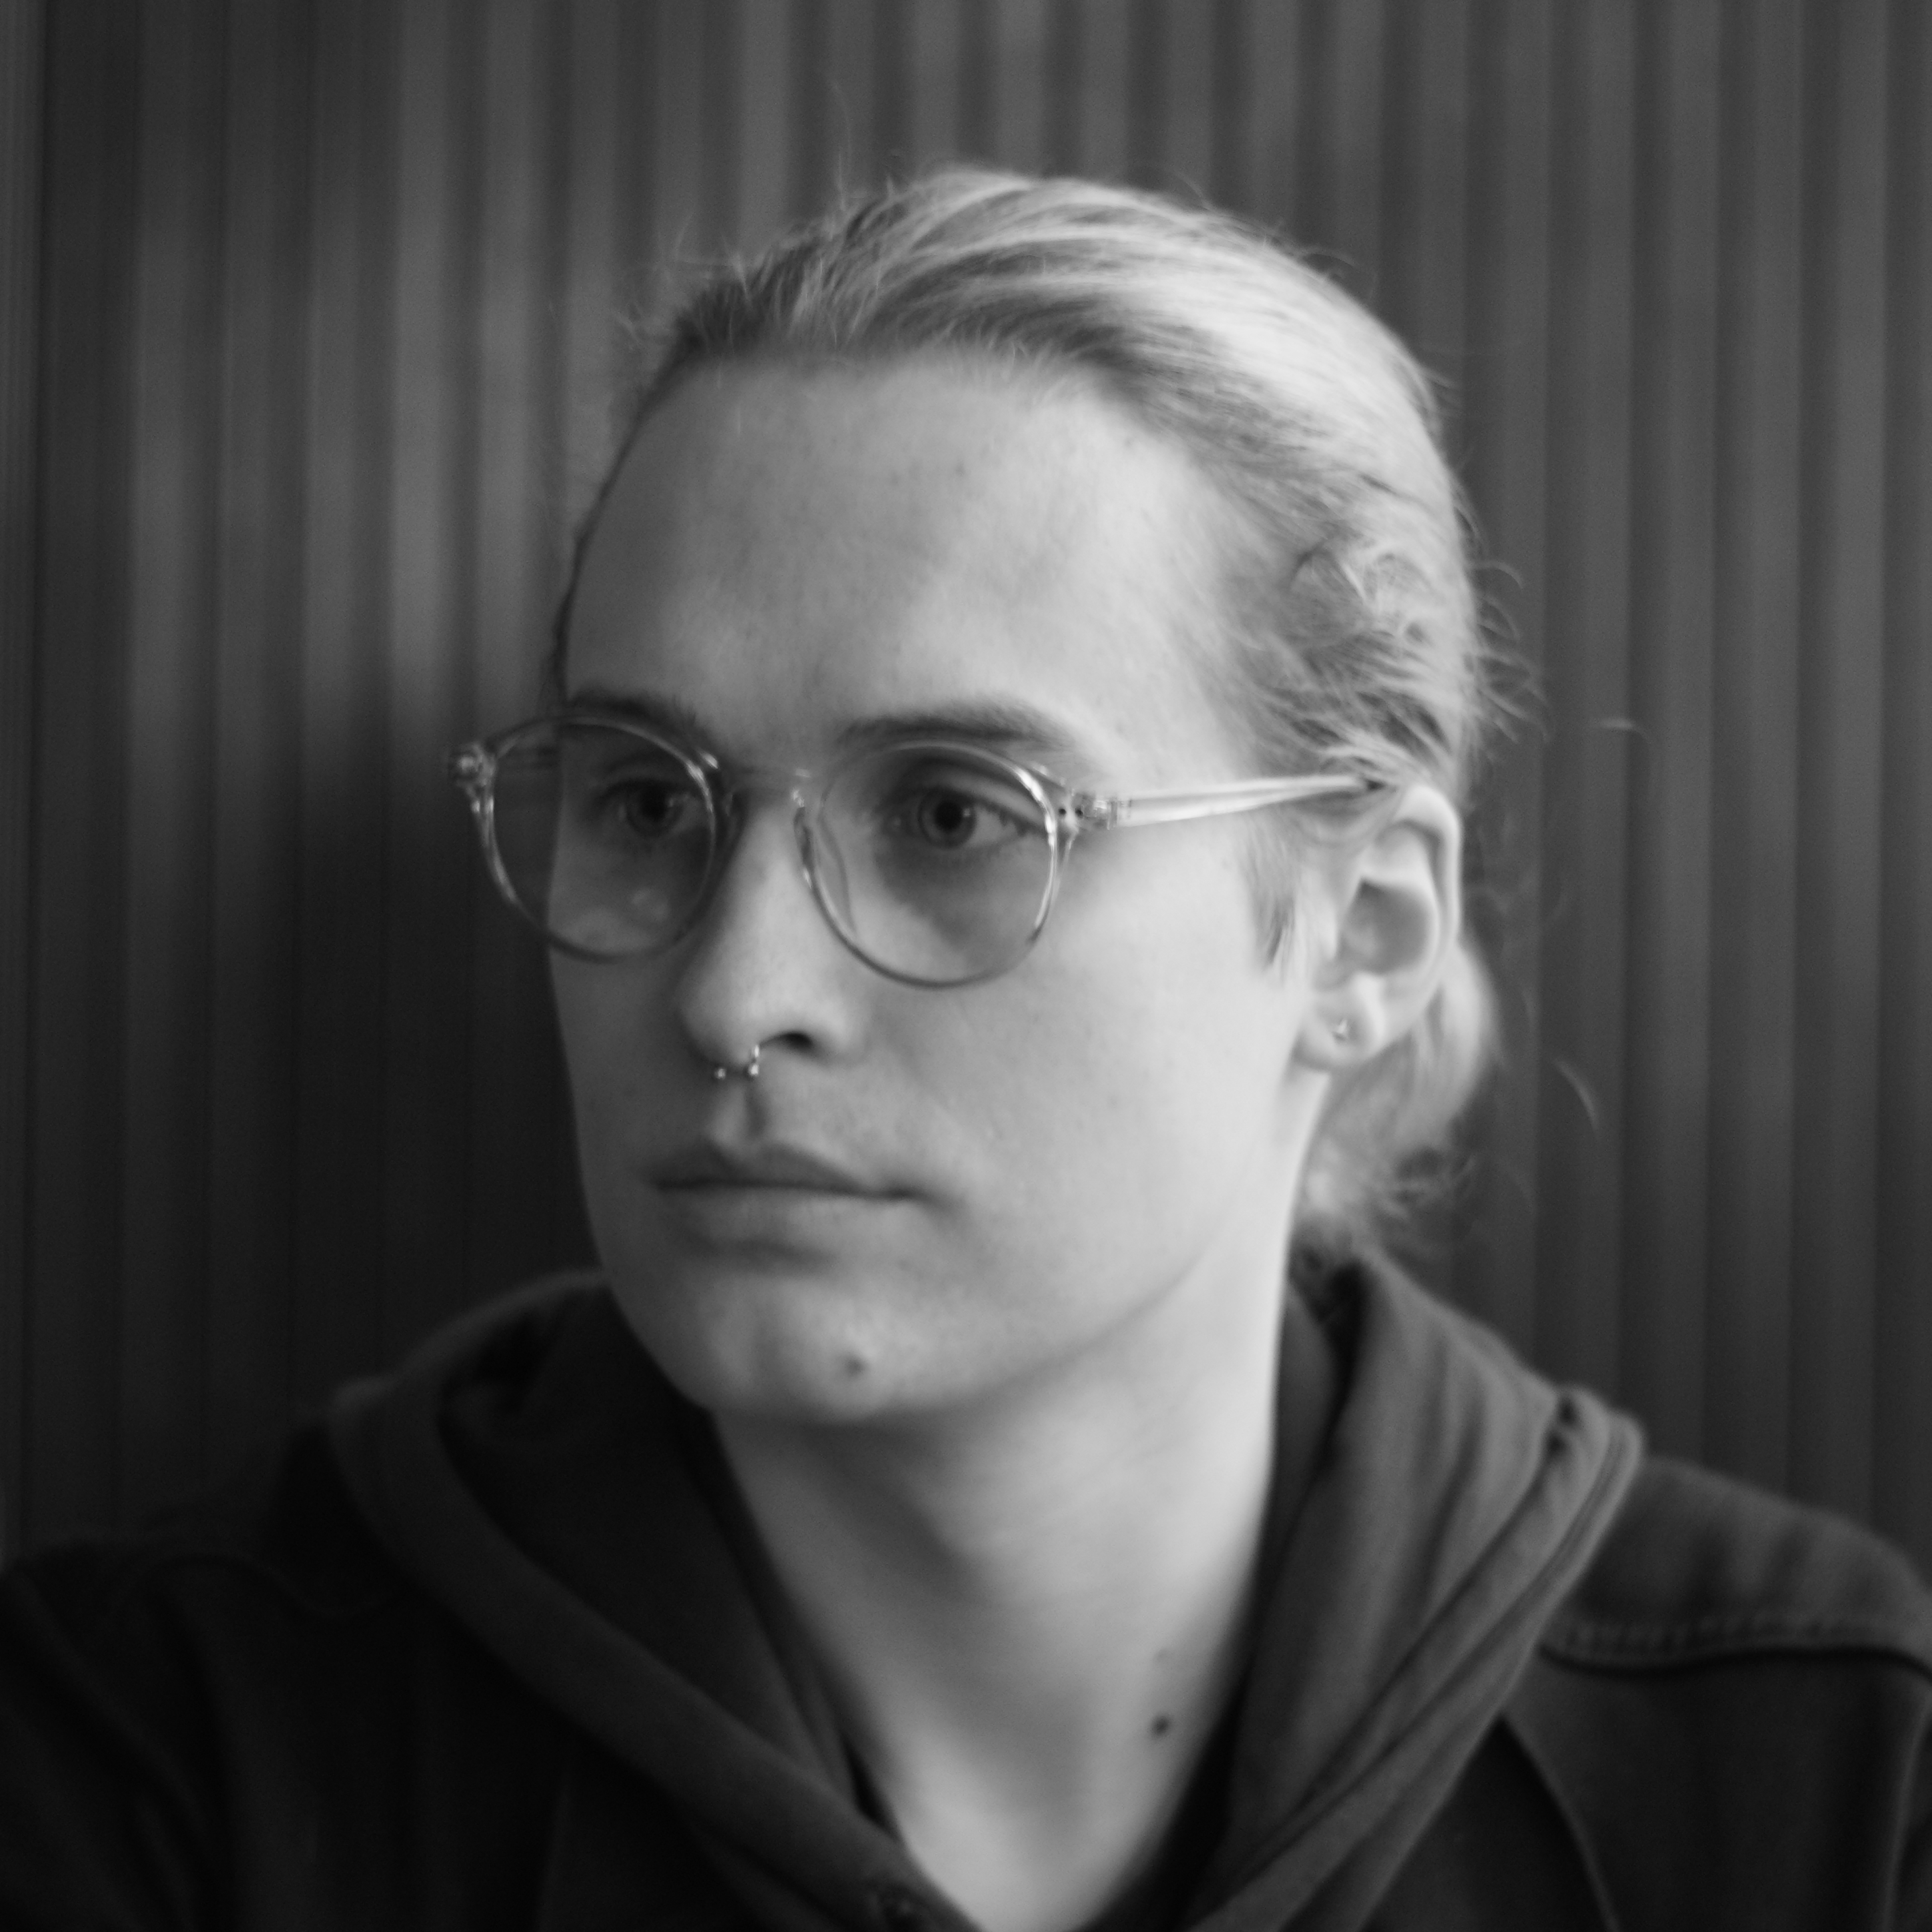
\includegraphics[width=4.0cm, keepaspectratio ]{Headshot.png}}; 
            \end{scope}
        \end{tikzpicture}
    \end{center}
    \vspace{20cm}
    \begin{center}
        \large{
            \color{white}{\faIcon{github} \href{https://github.com/aihphysics}{aihphysics}}\\
            \color{white}{\faIcon{link} \href{aihphysics.github.io}{aihphysics.github.io}}\\
            %%\color{white}{\faIcon{envelope} aihphysics@outlook.com}\\
            \color{white}{\faIcon{envelope} alina.hagan@cern.ch}\\
            %%\color{white}{\faIcon{twitter} \href{https://twitter.com/aihphysics}{@aihphysics}}\\
            %%\color{white}{\faIcon{linkedin} \href{https://www.linkedin.com/in/alina-hagan-3a62a6255/}{aihphysics}}\\
            \color{white}{\faIcon{map-marker-alt} CERN}\\
        }
    \end{center}
\end{bgbox}%
\begin{bgbox}[height=\paperheight,colback=gray,width=0.7\textwidth]
\small
    \vspace{0.6cm} 
    \flushleft
    \begin{description}
        \item \underline{Education}:
        \begin{description}
            \item[2020-2024] PhD, Lancaster University, ATLAS Experiment.
            \begin{itemize}
                \item Particle Physics, Supervised by Vato Kartvelishvili.
                \item Analysis Contact for Extracting Gluon TMDs from $J/\psi + \gamma$ in $pp$.
            \end{itemize}
            \item[2015-2020] MSc, University of Glasgow.
            \begin{itemize}
                \item First Class Masters in Physics.
                \item Masters project;
                \begin{itemize}
                    \item Measurement of $b$-jet substructure observables.
                    \item Exploration of novel overlap removal methods and Soft-Drop jet cleaning.
                \end{itemize}
            \end{itemize}
        \end{description}
        \item \underline{Experience}:
        \begin{description}
            \item[2022] ATLAS Collaboration
            \begin{itemize}
                \item BLS Trigger group.
                \item Authorship qualification project supervised by Adam Barton and Pavel Renicek.
                \item Updating ATLAS BLS Trigger Validation package and tools to Run 3 framework, expanding available tools and modernisations.
            \end{itemize}
            \item[2019] University of Glasgow.
            \begin{itemize}
                \item Nuclear and Hadron Physics research group.
                \item Supervised by Dr Simon Gardner.
                \item Appling GNNs for shower recognition at the Crystal Ball detector.
                \begin{itemize}
                    \item Utilising Graph Neural Network layers from \href{https://arxiv.org/abs/1902.07987}{1902.07987} and a YOLO-style approach to identify, separate and reconstruct overlapping showers.
                \end{itemize}
            \end{itemize}
        \end{description}
        \item \underline{Presentations \& conference}:
        \begin{description}
            \item[2023] {ATLAS Week, October 2023}
            \begin{itemize}
                \item Early Career Scientist Presentation - Exploring Proton Structure: Gluon TMDs at ATLAS
            \end{itemize}
            \item[2023] \href{https://indico.in2p3.fr/event/28579/}{Beauty 2023}
            \begin{itemize}
                \item New Heavy Flavour states in ATLAS
                \item $B$-Hadron reconstruction in early ATLAS Run 3 data
            \end{itemize}
            \item[2023] \href{https://indico.cern.ch/event/1213416/}{Quarkonia as Tools 2023}
            \begin{itemize}
                \item Inclusive quarkonium production - experimental overview. 
            \end{itemize}
            \item[2022] \href{https://indico.cern.ch/event/1077305/}{ATLAS UK Annual Meeting 2022}
            \begin{itemize}
                \item Precision physics with quarkonia.
            \end{itemize}
            \item[2022] \href{https://indico.cern.ch/event/1084752/}{Quarkonia as Tools 2022}
            \begin{itemize}
                \item Quarkonium and TMDs in pp - past and future measurements. 
            \end{itemize}
        \end{description}
        \item \underline{Academic Interests}:
        \begin{description}
            \item[Quarkonium Physics.]\; 
            \begin{itemize}
                \item $J/\psi$, Di-$J/\psi$, $J/\psi+\gamma$, $\Upsilon$ studies, TMD extraction.
            \end{itemize}
            \item[Trigger Development.]\; 
            \begin{itemize}
                \item Muon and b-physics trigger development, validation, and shift work.
            \end{itemize}
        \end{description}
        \item \underline{Projects}:
        \begin{description}
            \item[2022] \href{https://github.com/aihphysics/terminal_rendering}{terminal\_rendering}
            \begin{itemize}
                \item A simplified implementation of a rendering engine, with minimal dependencies, designed to work on any unicode compatible terminal.
            \end{itemize}
            \item[2023] \href{https://github.com/aihphysics/L1P}{Rockets}
            \begin{itemize}
                \item Designing and building 'L1' rockets. Two in-progress designs, minimum diameter and full body. Launches scheduled for november 2023.
            \end{itemize}
            \item[2023] \href{https://github.com/aihphysics/mini_neo_led_matrix}{PCB Design}
            \begin{itemize}
                \item Designing and building small form-factor neopixel-based smart LED boards for use with raspberry pi or arduino, and more.
            \end{itemize}
            %%\item[2022-NOW] FINITE STATE
            %%\begin{itemize}
            %%    \item A science fiction styled bridge operation game with an emphasis on complexity, technical knowledge of your craft, and operating procedure
            %%\end{itemize}
        \end{description}
    \end{description}
    \begin{description}
        \item \underline{Other}:
        \begin{description}
            \item[Skills] C++, Python, ROOT, CMake, Vim, Git, LaTeX, Laser cutter operation, 3D printing, Arduino and RP2040 programming.
            \item[Personal Information] Age - 25, Gender - Female, Nationality - Scottish.
            \item[Hobbies] Photography, running, maker activities.
        \end{description}
    \end{description}

\end{bgbox}

\end{document}
